While database systems have traditionally stored relational tables on a per-row
basis, recent developments have shown that a column-store format can outperform
traditional RDBMS for many workloads, particularly when the data fits into
main memory.
One of the first research prototypes of a column-based database manage systems
(DBMS) was MonetDB \cite{IdreosS2012}, still an active research project, but
many commercial systems now also support column-based storage (e.g.
Microsoft SQL Server~\cite{msqlserver},
SAP HANA~\cite{FarberF2012}, and
HyPer~\cite{Neumann2011:HyPer}).
% Microsoft SQL server
This fundamental shift in database architecture has resulted in a large body of
research efforts within the database community looking into efficient SQL query
execution on such a data format.

Given that in a column store each column of a table is stored as an array,
array programming languages appear as a promising construct to provide support
for query execution. In fact, \OldPaperAuthor introduced an intermediate
representation (IR) language, called \textit{HorseIR}, providing efficient
database operators.
\new{At the same time, it is a general-purpose high-level IR, and can therefore serve
not only as an effective representation for SQL but also other higher-level 
operators, pre-defined built-in functions, and other array-base languages such
as MATLAB. Thus, compared to existing query compilers that translate from relational
algebra to optimized code (e.g. Hyper), it is much more general and extensible.}
% \OldPaper shows very good results on standard database benchmarks.

SQL queries are first transformed into execution plans using standard database
optimization techniques that describe in which order and how database operators
such as joins, selections and aggregations should be executed depending on the
data to be analyzed. These execution plans are then translated into HorseIR,
the resulting code is optimized using techniques from array programming, and
finally the optimized code is compiled into multi-platform C code.

The approach used in HorseIR, however, does not take full advantage of the
optimization techniques available. Instead, it is restricted to basic code
fusion of element-wise operators, and although it explores some high-level
pattern-based optimization techniques, these require considerable knowledge of
database operators.  Optimization potential is also reduced by extensive use of
built-in functions, the complexity of which limits optimization.

For example, it is common for SQL queries to do a selection (selecting some
rows based on the filter criteria on one column) and then perform aggregation,
such as a summation.  In an array-based language this can be represented as

\begin{small}
\begin{Verbatim}[xleftmargin=.3\columnwidth]
R = sum(filter(C, A))
\end{Verbatim}
\end{small}

%%% $$
%%% R = sum(filter(C, A))
%%% $$

\noindent{}where the condition \texttt{C} is a boolean vector, the input array \texttt{A}
is a vector with the same number of elements, and the result \texttt{R} is a
scalar.  A straightforward way to generate C code from this is to generate two loops, the first applying the boolean selection and producing an intermediate result, and the second loop performing the reduction on this intermediate result.  A more optimized version, however, would fuse the two loops into one, performing the reduction on the fly and avoiding generation of an intermediate result:

\begin{center}
\begin{minipage}{\linewidth}
\begin{small}
\begin{lstlisting}[language=C, frame=single, xleftmargin=0mm, xrightmargin=5mm]
R=0;
for(int i=0; i<C.size; i++) {
    if(C[i]) { R += A[i]; } // true block
}
\end{lstlisting}
\end{small}
\end{minipage}
\end{center}

% add lines around box: frame=single
%\begin{small}
%\begin{Verbatim}[xleftmargin=.15\columnwidth]
%R=0;
%for(int i=0; i<C.size; i++) {
%    if(C[i]) { // true block
%        R += A[i];
%    }
%}
%\end{Verbatim}
%\end{small}

%%% \begin{lstlisting}[style=CStyle]
%%% for(int i=0; i<10; i++){
%%%     if(C[i]) { // true block
%%%         R += A[i]
%%%     }
%%% }
%%% \end{lstlisting}

%% However, HorseIR describes both sum and filter as built-in functions, and
%% currently no optimization across those functions can be performed.
\noindent{}The analysis required to generate such code from a series of built-in functions, however, is complex,
depending on non-trivial array dependency analysis as well as knowledge of array dimensions, and 
while possible in principle, our experience has been that these optimization opportunities are not found by our available C compilers.

% \refFig{fig:fusion_idea} shows that we propose automatic fusion which contains
% element-wise fusion and some parts of pattern-based fusion
% so that less pattern-based fusion is required.

\begin{figure}[htbp]
\centering
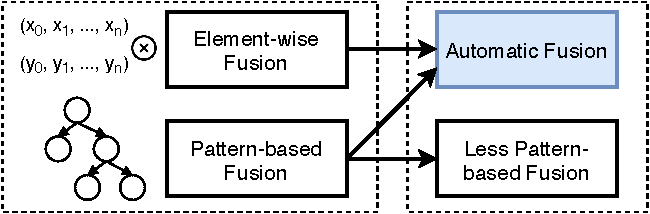
\includegraphics[width=.95\columnwidth]{./src/figure/basic-idea.pdf}
\caption{Automatic array-based (HorseIR) operator fusion for SQL queries includes element-wise fusion and a limited set of patterns.}
\label{fig:fusion_idea}
\end{figure}

In this paper we provide a systematic approach to analyze the SQL query programs
and generate optimized code. As shown in \refFig{fig:fusion_idea},
\textit{automatic fusion} is a blend of element-wise fusion and a limited set of
patterns. Including effective element-wise fusion allowed us to replace numerous fixed
patterns with a more general approach. More specifically, we provide a detailed
analysis of the most important built-in functions used for executing SQL operators
and explain how to optimize across such functions. Our approach is based on a
\textit{shape analysis}, which describes the layout and size of variables as
functions are applied. This allows us to fuse loops extensively, skip unnecessary
iterations over the data, and avoid intermediate results.  

% contribution
The contributions of this paper are summarized as follows:

\begin{itemize}
\item We explore a new approach to improve database query performance by
      applying techniques derived from array programming. We focus on HorseIR, an IR specifically designed to support database query execution.
\item We perform shape analysis on the built-in functions of HorseIR that represent database operators. This allows us to collect precise shape information and provide a conformability analysis to identify fusible sections in the HorseIR code. 
\item We present a set of optimization and code generation strategies to automatically
      generate optimized code.
\item We conduct experiments on the database benchmark TPC-H, to show the effectiveness of our technique.
\end{itemize}

\begin{comment}
The rest of this paper is organized as follows:
\refSec{Sec:background}
provides the background of HorseIR and array-based optimizations.
\refSec{Sec:overview}
introduces the description of the overview of our approach.
\refSec{Sec:shape}
presents our shape analysis for different groups of functions.
\refSec{Sec:conformability}
introduces our conformability analysis to identify fusible sections.
\refSec{Sec:codegen}
describes our code generation rules for generating efficient code.
\refSec{Sec:evaluation}
shows our experiments and experimental results.
\refSec{Sec:relatedwork}
discusses related work, and
\refSec{Sec:conclusion}
concludes.
\end{comment}
